\documentclass[]{politex}
% ========== Opções ==========
% pnumromarab - Numeração de páginas usando algarismos romanos na parte pré-textual e arábicos na parte textual
% abnttoc - Forçar paginação no sumário conforme ABNT (inclui "p." na frente das páginas)
% normalnum - Numeração contínua de figuras e tabelas 
%	(caso contrário, a numeração é reiniciada a cada capítulo)
% draftprint - Ajusta as margens para impressão de rascunhos
%	(reduz a margem interna)
% twosideprint - Ajusta as margens para impressão frente e verso
% capsec - Forçar letras maiúsculas no título das seções
% espacosimples - Documento usando espaçamento simples
% espacoduplo - Documento usando espaçamento duplo
%	(o padrão é usar espaçamento 1.5)
% times - Tenta usar a fonte Times New Roman para o corpo do texto
% noindentfirst - Não indenta o primeiro parágrafo dos capítulos/seções


% ========== Packages ==========
\usepackage[utf8]{inputenc}
\usepackage{amsmath,amsthm,amsfonts,amssymb}
\usepackage{graphicx,cite,enumerate}


% ========== Language options ==========
\usepackage[brazil]{babel}
%\usepackage[english]{babel}


% ========== ABNT (requer ABNTeX 2) ==========
%	http://www.ctan.org/tex-archive/macros/latex/contrib/abntex2
%\usepackage[num]{abntex2cite}

% Forçar o abntex2 a usar [ ] nas referências ao invés de ( )
%\citebrackets{[}{]}


% ========== Lorem ipsum ==========
\usepackage{blindtext}



% ========== Opções do documento ==========
% Título
\titulo{Sistema Web para Instalação de ERBs}

% Autor
\autor{Eric Rodrigues Pires \\%
       Mateus Nakajo de Mendonça}

% Para múltiplos autores (TCC)
%\autor{Nome Sobrenome\\%
%		Nome Sobrenome\\%
%		Nome Sobrenome}

% Orientador / Coorientador
\orientador{Bruno de Carvalho Albertini}
%\coorientador{Nome do coorientador (opcional)}

% Tipo de documento
\tcc{de Computação}
%\teseDOC{Engenharia Elétrica}
%\teseLD
%\memorialLD

% Departamento e área de concentração
\departamento{PCS}
%\areaConcentracao{Área de concentração}

% Local
\local{São Paulo}

% Ano
\data{2018}




\begin{document}
% ========== Capa e folhas de rosto ==========
\capa
\falsafolhaderosto
\folhaderosto


% ========== Folha de assinaturas (opcional) ==========
%\begin{folhadeaprovacao}
%	\assinatura{Prof.\ X}
%	\assinatura{Prof.\ Y}
%	\assinatura{Prof.\ Z}
%\end{folhadeaprovacao}


% ========== Ficha catalográfica ==========
% Fazer solicitação no site:
%	http://www.poli.usp.br/en/bibliotecas/servicos/catalogacao-na-publicacao.html


% ========== Dedicatória (opcional) ==========
\dedicatoria{Dedicatória}


% ========== Agradecimentos ==========
\begin{agradecimentos}

Thanks...

\end{agradecimentos}


% ========== Epígrafe (opcional) ==========
\epigrafe{%
    \emph{``Epígrafe''}
    \begin{flushright}
        -{}- Autor
    \end{flushright}
}


% ========== Resumo ==========
\begin{resumo}
Este projeto de formatura tem como objetivo criar um sistema capaz de calcular
posições para a instalação de Estações Radiobase (ERBs) de forma que a
cobertura da rede de ERBs seja máxima. A partir da região dada como entrada, o
sistema obterá seus dados geográficos através de um Sistema de Informações 
Geográficas (SIG) e utilizará programação específica para a otimização da posição
de instalação. Para interface com o usuário do sistema, criaremos uma aplicação
Web responsiva que permita selecionar a região na qual se pretende instalar uma
ERB e mostra as posições ideais para instalação.
\\[3\baselineskip]
%
\textbf{Palavras-Chave} -- Estações~Radiobase, Otimização, Sistema~de~
Informações~Geográficas, Aplicação~Web.
\end{resumo}


% ========== Abstract ==========
\begin{abstract}
This term paper intends to achieve a system capable of calculating the position
to install cellular Base Stations (BS) so that we maximize the coverage network.
From a given input region, the system will collect geographic data through a
Geographical Information System (GIS) and utilize specific programming to optimize
the placement position. For interfacing with the system user, we will develop a
responsive Web application that allows the selection of a region on which we
intended to place a BS, and show the ideal points for installation.
\\[3\baselineskip]
%
\textbf{Keywords} -- Base~Stations, Optimization, Geographical~Information~
System, Web~Application.
\end{abstract}


% ========== Listas (opcional) ==========
\listadefiguras
\listadetabelas

% ========== Listas definidas pelo usuário (opcional) ==========
\begin{pretextualsection}{Lista de símbolos}

\textbf{ERB:} Estação Radiobase

\textbf{SIG:} Sistema de Informações Geográficas

\end{pretextualsection}

% ========== Sumário ==========
\sumario



% ========== Elementos textuais ==========

\chapter{Introdução}
Na revolução da informação em que vivemos hoje, em que cada vez mais pessoas
estão conectadas à rede, o acesso à Internet tem se tornado cada vez mais
essencial no dia-a-dia, até mesmo a populações consideradas isoladas. Empresas
bem conhecidas, como Vivo e Claro, vêm se empenhando para garantir melhor
acesso a mais pessoas, mas se deparam com problemas de engenharia nesta
tarefa.

A extensão territorial e a densidade demográfica desigual do Brasil são dois
dentre vários fatores que tornam problemas de telecomunicação mais complexos.
A dimensão deste problema gera um grande potencial de mercado para empresas
terceirizadas, voltadas à instalação de Estações Radiobase (ERBs) para
compartilhamento ou aluguel de células telefônicas às grandes empresas de
telecomunicação. Dessa forma, há demanda do mercado por ferramentas que
simplifiquem e/ou automatizem a tarefa de estudo de localização de ERBs.

\section{Objetivo}
O objetivo deste projeto de formatura é criar um sistema que permita calcular
posições para a instalação de antenas de telefonia de forma a maximizar o
alcance delas. Com esse fim, levaremos em conta dados geográficos para
realizarmos os cálculos.

Também é de grande importância que tal sistema tenha uma interface prática
para os usuários. Portanto, uma interface web que apresente os dados
requisitados é essencial para o projeto.

Outras possíveis ramificações do projeto para showcase ao público geral, que não
é o público-alvo, é a localização de antenas a partir do próprio celular do
usuário, e a estimativa de posição do dispositivo pelas antenas encontradas.

\subsection{Sistema de Informação Geográfica}
Um SIG (Sistema de Informação Geográfica) é um sistema computacional capaz de
obter, gravar, gerir, analisar e visualizar dados geográficos. Seu uso permite
tomar decisões, analisar estatísticas e resolver problemas de otimização a
partir de dados geográficos. O SIG pode ser usado tanto em lojas de varejo para
decidir onde abrir uma nova filial, como em rastrear padrões de migração,
controle e o monitoramento do desmatamento, planejamento urbano, etc.

No nosso projeto, usaremos um software SIG para gravar e exibir a posição de
ERBs (Estações Radiobase) atuais, o relevo e os consumidores atingidos pela
rede de ERBs. Com essas informações, determinaremos as posições ótimas de
ERBs de modo a maximizar a área de cobertura do sistema de telefonia.
Para tanto, aplicaremos técnicas de programação linear, uma vez que
estamos diante de um problema de otimização cuja função a ser otimizada
é linear em relação às variáveis de entrada.

\subsection{Interface Web}
Para interação com o usuário, criaremos um front-end de uma aplicação Web que
permita selecionar a região na qual se pretende instalar alguma ERB.
Esta interface se comunicará com o back-end do SIG, para obter e calcular os
dados desejados.

O design deverá ser responsivo, podendo ser utilizado em plataformas mobile
ou desktop, e simples, com opções simples para apenas verificar a posição ótima
de instalação de antenas em determinada área escolhida pelo usuário. Para isso,
a interface deverá exibir um mapa, como por exemplo o da plataforma
OpenStreetMap, com as informações do SIG, que permita ao usuário selecionar uma
área desejada. Os dados serão calculados no back-end e exibidos ao usuário na
tela. Para isso, será necessário desenvolver um front-end possivelmente
dinâmico.

\section{Motivação}
Com uma análise preliminar do setor, verificamos o mercado de instalação e
aluguel de torres telefônicas no Brasil para comparar as tecnologias utilizadas
em softwares ou pesquisas de  de ERBs. Há várias técnicas empregadas, desde
programação não-linear a algoritmos evolutivos, algoritmos de polinização a
programação inteira mista. Será feita uma comparação das tecnologias para
verificar a que mais se adequa ao nosso caso de uso.

Também pesquisamos serviços similares da concorrência. Um dos
produtos encontrados, chamado Atoll, é um software de planejamento de células e
posições de ERBs, similar ao que desejamos desenvolver, porém com 
funcionalidades extendidas como manutenção e melhoria de locais 
pré-estabelecidos, e parâmetros avançados de especificação das antenas, além de
módulos para outras tecnologias de telecomunicação como Wi-Fi \cite{atoll}.
Porém, a ferramenta parece muito voltada à instalação urbana e análise de
infra-estrutura pré-existente, sem foco em uma eventual expansão. Por isso,
vemos como que há necessidade do mercado por uma ferramenta voltada à ampliação
de uma rede de ERBs.

\section{Justificativa}
Sobre potenciais clientes, verificamos a existência de empresas no Brasil para
localizar antenas, alugar terrenos para a instalação de antenas ou alugar
antenas para empresas de telecomunicação. A maior parte destas empresas foca em
um contexto urbano, enquanto que há interesse das empresas de telecomunicação
e dos governos estaduais em expansão em áreas rurais.

MyTower é um portal de locação e venda de imóveis para operadoras de
telecomunicação \cite{mytower}. Ele permite que o usuário cadastre seu imóvel
e o anuncie para as operadoras após aprovação.
O portal então faz a intermediação entre o anunciante e a operadora.

A Skysites é uma empresa que oferece soluções na área da infraestrutura de
telecomunicação \cite{skysites}. Ela gere um portifólio de sítios para 
instalação de equipamentos de telecomunicação (torres, smallcells, rooftops,
etc), além de prover soluções customisadas para empresas de telecomunicação e 
compartilhar torres entre diferentes empresas. Outros serviços são redes para
cobertura \textit{indoor} e pequenas ERBs para melhorar a cobertura em ambiente
urbano, as \textit{small cells}.

\section{Organização do Trabalho}
No capítulo ``Introdução" deste trabalho, definimos a motivação da realização
deste sistema e o que buscamos alcançar neste projeto.

No capítulo ``Aspectos Conceituais'', será realizada a contextualização dos
conceitos empregados na área de aplicação e a revisão da literatura de base.

No capítulo ``Tecnologias Utilizadas'', listaremos as ferramentas, algoritmos
e dados necessários para o desenvolvimento do sistema deste trabalho.

No capítulo ``Metodologia do Trabalho'', definiremos os processos e fases
no desenvolvimento de funcionalidades deste sistema, como concepção, estudo,
projeto, implementação e testes.

No capítulo ``Especificação de Requisitos do Sistema'', definiremos os
requisitos do nosso sistema.

\chapter{Aspectos Conceituais}

\section{Algoritmos Avaliados}
Em consulta à literatura pré-existente sobre o problema de otimização de
instalação de ERBs, nos deparamos com várias abordagens distintas para o mesmo
problema, em diferentes níveis de abstração.

A princípio, nós nos voltamos a duas alternativas: LEE~et~al.~(2015)~
\cite{evolutivo} utiliza conceitos básicos de telecomunicações, através de uma
fórmula para calcular a satisfação dos usuários do sistema a partir de medidas
de qualidade de banda, se baseando em um algoritmo evolutivo para otimizar
a cobertura da rede. Já KARULKAR~\&~OH~(2016)~\cite{nao-linear} se baseia em
uma abordagem de limites geográficos impostos no processo de projeto de antenas,
utilizando programação não-linear para identificar a posição ótima.

\chapter{Tecnologias Utilizadas}

\section{Framework Web Django}
No projeto, para facilidade de desenvolvimento, utilizaremos o framework Django,
escrito em Python. A integração de single-page com o back-end deverá ser feita
com o módulo de API REST do Django.

O Django possui funcionalidades de SIG pelo módulo GeoDjango, que utiliza como
banco de dados o PostGIS (baseado em Postgres). Serão armazenados
dados públicos de localização de ERBs, relevo e densidade populacional. Ele
será também responsável pelos cálculos realizados para a localização de novas
antenas.

Para interação com o usuário por um mapa interativo, utilizaremos a biblioteca
Leaflet, escrita em JavaScript. Ela se comunicará aos dados pela API REST a ser
desenvolvida, tanto para requisições quanto para exibições.

\section{Bases de Dados Utilizadas}
Utilizamos o Mapa de ERBs Brasil presente no portal Telebrasil \cite{mapa-erb}.
Essa base contém uma lista de ERBs do Brasil de novembro de 2017, com
informação de operadora, endereço, e posição geográfica de cada ERB.
Essas infomações são essenciais para o cálculo da posição ótima da ERB para
maximizar a cobertura da célula.

Utilizamos também o OpenCelliD, da empresa Unwired Labs \cite{opencellid}.
Essa base contém uma lista de ERBs do mundo inteiro, com o CGI de cada ERB.
Os dados foram obtidos através da colaboração de usuários do aplicativo
LocationAPI da Unwired Labs. O LocationAPI trata-se de um serviço de
geolocalização que não depende de GPS. Dessa forma, com a base da OpenCelliD,
podemos estimar a posição de um celular a partir das ERBs as quais ele está
conectado.

Outra base de dados em estudo foi o Google Earth Engine, uma API específica
para dados geográficos públicos do Google, como relevo e densidade populacional.
Devido à extensão destes dados, será estudada a possibilidade de uma dependência
desta base.

\chapter{Metodologia do Trabalho}
Em uma primeira etapa, definimos com o orientador a proposta e o escopo deste
projeto, propondo a pesquisa a ser realizada tanto da perspectiva de
implementações quanto de requisitos necessários. Levantados tais requisitos no
capítulo ``Especificação de Requisitos do Sistema'', a próxima etapa se baseou
em projetar a realização de cada um destes requisitos de acordo com as
prioridades definidas, isto é, iniciar um processo de decisões definitivas para
o andamento do trabalho.

\chapter{Especificação de Requisitos do Sistema}
Para definir os requisitos do nosso sistema, foi elaborada uma árvore de
pré-requisitos, listando a prioridade total dada a cada componente do sistema
final na Figura~\ref{fig:arvore_prerequisitos}.

\begin{figure}
  \centering
  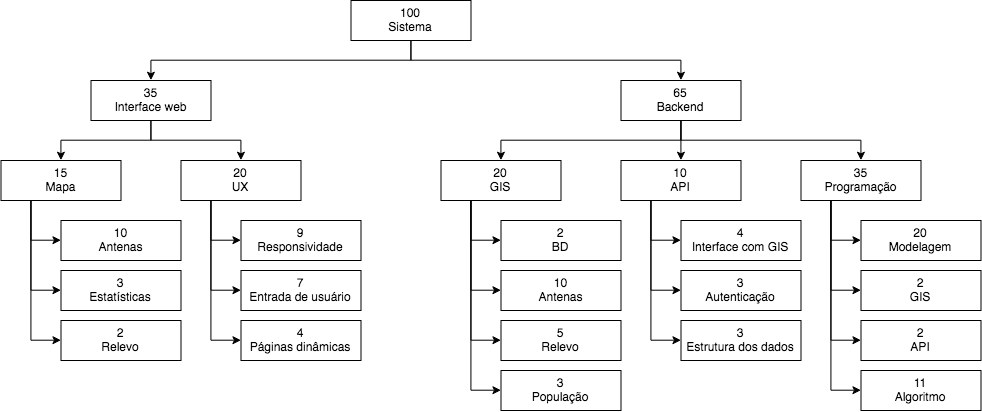
\includegraphics[width=5.5in]{imagens/arvore_prerequisitos}
  \caption{Árvore de pré-requisitos do sistema.}
  \label{fig:arvore_prerequisitos}
\end{figure}

Como evidenciado pela figura, a ênfase deste projeto será no back-end, em
especial na parte de modelagem e programação relacionadas ao cálculo de
otimização da posição de antenas. As outras duas partes relevantes do 
\emph{backend} tratam, respectivamente, do uso do banco de dados como SIG e da
comunicação externa de dados via API.

Embora tenha uma ênfase menor, o front-end da interface web também será
um requisito fundamental de projeto, separado na experiência do usuário e na
visualização do mapa.

\chapter{Projeto e Implementação}

\chapter{Testes e Avaliação}

\chapter{Considerações Finais}
\section{Conclusões do Projeto de Formatura}
\section{Contribuições}
\section{Perspectivas de Continuidade}



% ========== Referências ==========
% --- IEEE ---
%	http://www.ctan.org/tex-archive/macros/latex/contrib/IEEEtran
%\bibliographystyle{IEEEbib}

% --- ABNT (requer ABNTeX 2) ---
%	http://www.ctan.org/tex-archive/macros/latex/contrib/abntex2
%\bibliographystyle{abntex2-num}

\begin{thebibliography}{9}
    
    \bibitem{atoll}
    Forsk.
    \textit{Atoll LTE / LTE-A Planning Software | Forsk}
    Disponível em: http://www.forsk.com/ltelte-pro
    Acesso em: 01º de março de 2018.

    \bibitem{mytower}
    MyTower.
    \textit{MyTower - Aluguel e Venda de Terrenos e Topos para
    Operadoras de Telecom}
    Disponível em: http://www.mytower.com.br/
    Acesso em: 01º de março de 2018.

    \bibitem{skysites}
    Skysites.
    \textit{Skysites}
    Disponível em: http://skysites.com/
    Acesso em: 01º de março de 2018.

    \bibitem{mapa-erb}
    Telebrasil.
    \textit{Mapa de ERBs Brasil (antenas)}.
    Disponível em:
    http://www.telebrasil.org.br/panorama-do-setor/mapa-de-erbs-antenas.
    Acesso em: 31 de janeiro de 2018.

    \bibitem{opencellid}
    Unwired Labs.
    \textit{OpenCelliD - Largest Open Database of Cell Towers \&
    Geolocation by Unwired Labs}.
    Disponível em: https://opencellid.org/
    Acesso em: 01º de março de 2018.

    \bibitem{evolutivo}
    LEE, S.; LEE, S.; KIM, K.; KIM, YH.
    \textit{Base Station Placement Algorithm for Large-Scale LTE
    Heterogeneous Networks}.
    PLoS ONE 10(10), 2015.

    \bibitem{nao-linear}
    KARULKAR, S. A.; OH, JY.
    \textit{Optimal Placement of Base Station for Cellular Network Expansion}.
    Issues in Information Systems, volume 17, edição II, pg. 215-221, 2016.

\end{thebibliography}
% ========== Apêndices (opcional) ==========
\apendice


% ========== Anexos (opcional) ==========
\anexo



\end{document}
\grid
\grid
